\documentclass[oneside,reqno]{amsart}
\setlength{\textwidth}{\paperwidth}\addtolength{\textwidth}{-2in}\calclayout
\usepackage[utf8]{inputenc}
\usepackage{enumitem}
\usepackage{tikz}
\usepackage{minted}\newminted{python3}{frame=lines}
\usepackage{booktabs}
\usepackage{etoolbox}
\makeatletter
\patchcmd{\@sect}{%
   \ignorespaces#8\unskip\@addpunct.}{\ignorespaces#8\unskip}{}{}
\makeatother
\allowdisplaybreaks[1]
\usepackage[normalem]{ulem}
\useunder{\uline}{\ul}{}

\DeclareMathOperator{\E}{E}
\DeclareMathOperator{\var}{var}
\DeclareMathOperator{\cov}{cov}
\DeclareMathOperator{\corr}{corr}
\DeclareMathOperator{\tr}{tr}
\DeclareMathOperator{\diag}{diag}
\DeclareMathOperator{\rank}{rank}
\let\vec\relax\DeclareMathOperator{\vec}{vec}
\let\vech\relax\DeclareMathOperator{\vech}{vech}
\newcommand{\eps}{\varepsilon}
\newcommand{\ups}{\upsilon}
\newcommand{\N}{\mathrm N}

\theoremstyle{definition}
\newtheorem{prob}{Problem}
\renewcommand*{\proofname}{Solution}
\setlist[enumerate]{label={(\roman*)}}
\title{ECON 706: Problem Set 2}
\author{Daniel Pfeffer}
\date{\today}
%------------------------------------------------------------------------------
\begin{document}
\maketitle

\begin{prob}
Download monthly U.S. housing starts and completions from the database of the St. Louis Fed. Use data beginning from January 1970. Graph and discuss the data.
\end{prob}

\begin{proof}
Figure \ref{plot-series} displays U.S. housing starts and completions measured in thousands of units from January 1970 until January 2020. Both series show evidence of cyclical components. Starts and completions tend to rise during periods of economic expansion and fall during economic slowdown. For example, during the Great Recession in 2008, housing starts and completions fell to an all time low, increasing over the subsequent years. Another characteristic displayed by these series is the tendency for completions to lag starts; an increase in starts is often followed by an increase in completions, and a decrease in starts if often followed by a decrease in completions.
\begin{figure}
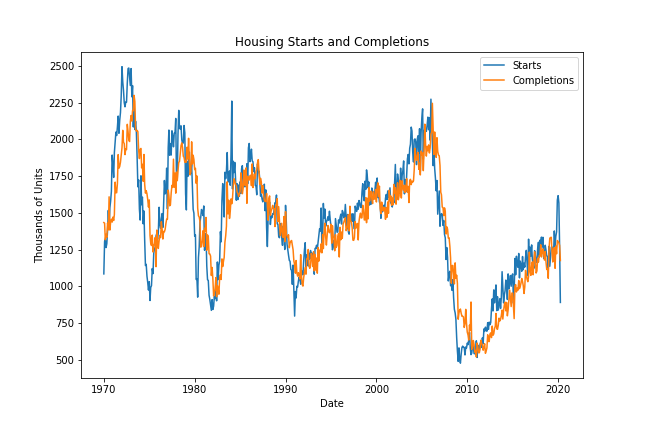
\includegraphics[width=\textwidth]{plot-series}
\caption{U.S. housing starts and completions from January 1970 until January 2020.}
\label{plot-series}
\end{figure}
\end{proof}

\begin{prob}
Using all data but the last 12 observations (reserved for out-of-sample forecast comparisons), estimate the two series jointly as a VAR(4).
\end{prob}


\begin{proof}
Prior to estimation, the joint series were partitioned into a training set and a test set containing the last 12 observations. The two series were then jointly estimated as a VAR(4), and the results are summarized in Figure \ref{var-summary}. We first analyze the results for the starts equation. The coefficients on the first three lags of starts are positive and significant (the $p$-values are all less than 0.005). The coefficient on the fourth lag is insignificant. Moreover, all four coefficients on completions are each not significantly different from zero. Next, we analyze the completions equation. All of the coefficients on the first four lags of completions are positive and significant. Moreover, the first, third, and fourth lags on starts have positive and significant coefficients. Only the constant and the coefficient on the second lag of starts are insignificant. 

\begin{table}
\caption{VAR(4) results.}
\begin{center}
\begin{tabular}{lcc}
\hline
          	        		& Starts & Completions  \\
\midrule
L1.Starts                    & 0.631*** & 0.078***  \\
                                  & (0.169)   & (0.028) \\
L1.Completions		& -0.002     & 0.279***  \\
            	       		& (0.064)   & (0.042) \\
L2.Starts    		& 0.277*** & 0.024 \\
          	       		& (0.050)   & (0.032) \\
L2.Completions    	& -0.084    & 0.200*** \\
          	       		& (0.066)   & (0.043) \\
L3.Starts			& 0.141*** & 0.068* \\
          	       		& (0.050)   & (0.033) \\
L3.Completions   	& -0.025    & 0.091* \\
          	       		& (0.064)   & (0.042) \\	       
L4.Starts			& 0.015     & 0.085*** \\
          	       		& (0.046)   & (0.030) \\
L4.Completions   	& 0.043     & 0.169*** \\
          	       		& (0.058)   & (0.038) \\	
\hline
Standard errors in parentheses. \\
* $p<.1$, ** $p<.05$, *** $p<.01$
\end{tabular}
\end{center}
\label{var-summary}
\end{table}
\end{proof}

\begin{prob}
Compute the autocorrelation function implied by your estimation. Plot the auto- and cross-correlations for different lags. 
\end{prob}

\begin{proof}
Figure \ref{acf-plots} contains autocorrelation and cross-correlation plots out to 25 lags. The upper left plot is the autocorrelation function of starts on starts, and it displays slow geometric decay. Similarly, the lower right plot is completions on completions, and also displays slow geometric decay. The lower left plot is the cross-correlation function of completions on starts. It displays contemporaneous correlation (at lag 0) of around $0.80$, rising to a maximum from around lag 6 to lag 9, then slowly decaying. This pattern is likely related to the fact that take around 6-9 months to build, hence it is not unexpected that we see an increase correlation around lag 6 to lag 9. Finally, the upper right plot is the cross-correlation function of starts on completions. It decays geometrically, and lacks the hump-shaped patters previously observed. This may be related to the fact that completing a house is less strongly indicative of another house being started.
\begin{figure}
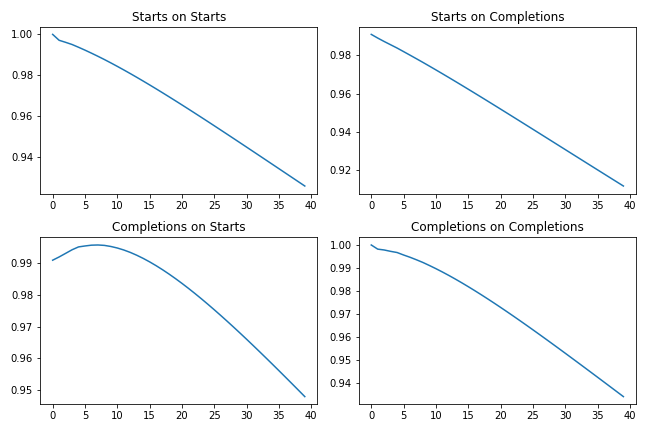
\includegraphics[width=\textwidth]{acf-plots}
\caption{Autocorrelation and cross correlation functions implied by the estimated VAR(4).}
\label{acf-plots}
\end{figure}

\end{proof}

\begin{prob}
Compute the spectral density function (SDF). Plot the univariate SDFs as well as the coherence.
\end{prob}


\begin{proof}
Figure \ref{sdf} contains plots for the starts and completions spectral density functions and the coherence between these two time series. Both of the univariate spectral densities peak at low frequencies, indicating that the variance in both of the series is attributable to the low frequency components. Moreover, the coherence has its first and largest peak at a low frequency, indicating that they are jointly influenced by frequencies at this low cycle. A potential explanation of the second peak in the coherence around $\pi/2$ may correspond to our earlier comment that housing starts typically imply a completions around 6-9 months later. 
\begin{figure}[!h]
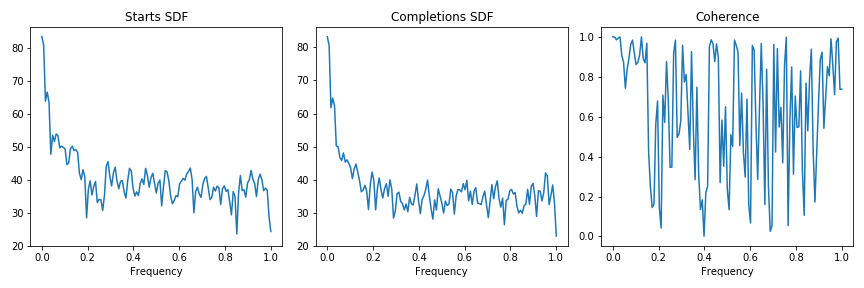
\includegraphics[width=\textwidth]{sdf}
\caption{}
\label{sdf}
\end{figure}
\end{proof}

\begin{prob}
Perform a Granger-causality analysis.
\end{prob}

\begin{proof}
We first test the null hypothesis that starts do not Granger-cause completions. Table \ref{granger} shows the results for an $F$-test of this null hypothesis. We reject null hypothesis at a 5\% significance level and conclude that starts Granger-cause completions, as expected based on our intuition.
\par
Next we test the null hypothesis that completions does not Granger-cause starts. Table \ref{granger} shows the results for an $F$-test of this null hypothesis. We reject null hypothesis at a 5\% significance level and conclude that completions Granger-cause starts. Hence, the system displays feedback.
\begin{table}
\caption{Granger-causality analysis.}
\begin{tabular}{lcccc}
\hline
	Null Hypothesis & Test Statistic & Critical Value & $p$-value  \\
\midrule
       \text{Starts does not cause completions} & 47.34  & 2.380  & 0.000   \\ 
       \text{Completions does not cause starts}  & 1.617 &  2.380 & 0.168  \\
\hline
\end{tabular}
\label{granger}
\end{table}
\end{proof}


\begin{prob}
Using Cholesky factor identification, compute the impulse-response functions (IRFs) as well as the variance decompositions. Graph the IRFs.
\end{prob}

\begin{proof}
Figure \ref{irf} shows orthogonalized impulse response functions. On the upper left, we see that a unit shock to starts results in an initial increase to starts at around 100 units and levels off at around 65 units. On the upper right, we see that a unit shock to completions has a minimal impact on starts, which can be seen by the large confidence intervals that contain both positive and negative numbers. On the lower right, we see that a unit shock to starts results in first a minor increase to completions, which increases further at around lag 4. This is likely related to time it take to build a house. Finally on the lower left, we see that a shock to completions results in an initial increase to completions that goes to zero at around lag 9. 
\begin{figure}
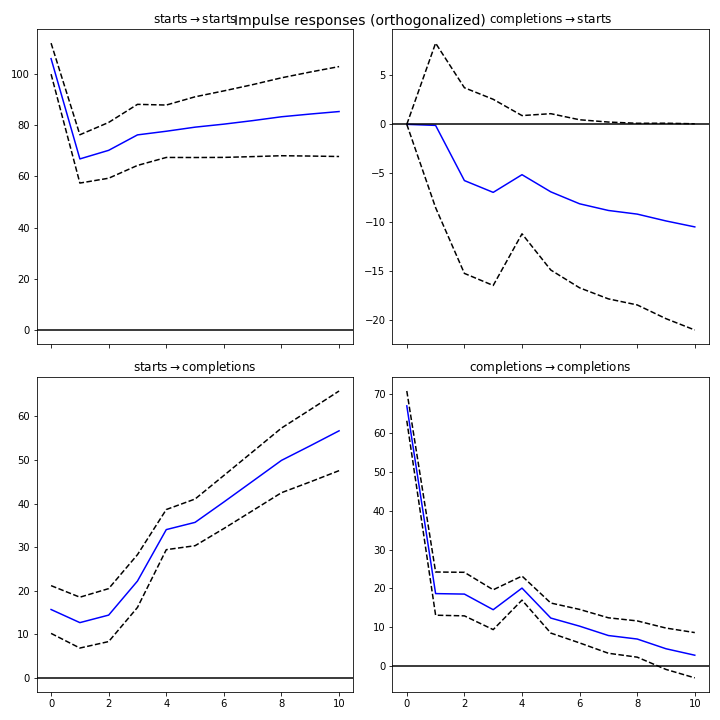
\includegraphics[width=\textwidth]{irf}
\caption{Orthogonalized impulse response functions.}
\label{irf}
\end{figure}
\begin{table}
\caption{Forecast error variance decomposition results.}
\begin{tabular}{lllll}
 & \multicolumn{2}{c}{{\ul Starts FEVD}} & \multicolumn{2}{c}{{\ul Completions FEVD}} \\
Horizon & Starts & Completions & Starts & Completions \\ \hline
0 & 1.000000  & 0.000000  & 0.052131 & 0.947869 \\
1 &  0.999999   &  0.000001 & 0.077790  & 0.922210  \\
2 &  0.998405    & 0.001595   & 0.106267  & 0.893733  \\
3 &  0.996939   &  0.003061  &  0.170836  &   0.829164  \\
4 &  0.996697  &   0.003303  &  0.281572   & 0.718428  \\
5 &  0.996013   &  0.003987  &  0.373584  &   0.626416  \\
6 &  0.995139  &   0.004861  &   0.461076  &   0.538924  \\
7 &  0.994288   &  0.005712  &  0.541396   &  0.458604  \\
8 &  0.993548  &   0.006452  &   0.611799  &   0.388201  \\
9 &  0.992784  &   0.007216  &  0.670018  &   0.329982 \\ \hline
\end{tabular}
\label{fevd}
\end{table}
\end{proof}

\begin{prob}
Forecast the 12 held-out observations and assess accuracy. Provide not only point forecasts, but also some measure(s) of uncertainty.
\end{prob}

\begin{proof}
Figure \ref{forecast} shows 12-step ahead forecasts for starts and completions with 2 standard error confidence bands. We predict an increase in both starts and completions. However, it should be noted that the variability in both of these forecasts increase sharply with the forecast horizon, as can be seen the the 2 standard error confidence bands. 
\begin{figure}
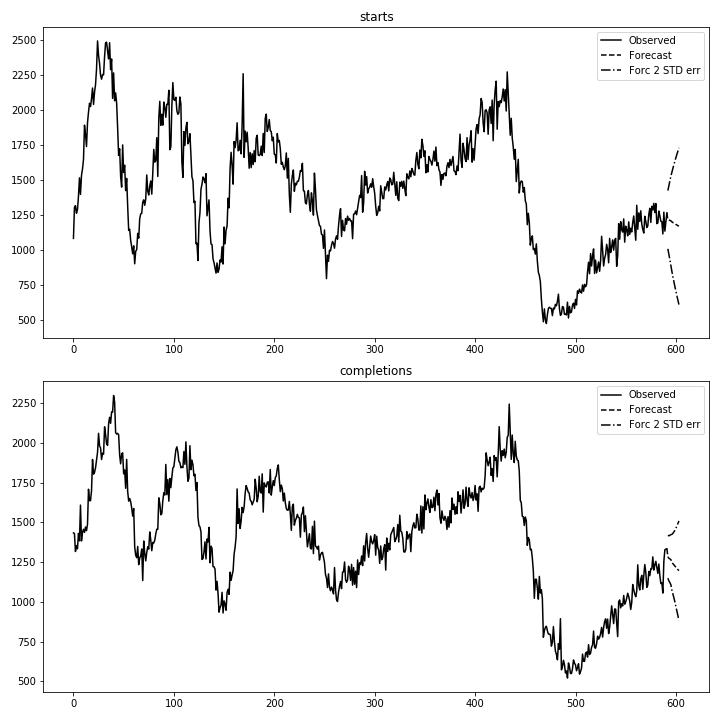
\includegraphics[width=\textwidth]{forecast}
\caption{}
\label{forecast}
\end{figure}
\end{proof}


\subsection*{Appendix}

The code used to generate the above results is presented below. 
\begin{python3code}
import numpy as np
import matplotlib.pyplot as plt
from statsmodels.tsa.api import VAR
from numpy.fft import fft
import pandas_datareader.data as web
import datetime

# 1984:Q1 to 2015:Q4
start = datetime.datetime(1970, 1, 1)
end = datetime.datetime(2020, 4, 1)

# Quarterly U.S. real GDP from the FRED
ts = web.DataReader(['HOUST', 'COMPUTSA'], 'fred', start, end)
ts = ts.rename(columns={'HOUST':'starts', 'COMPUTSA': 'completions'})

# Plot series
plt.figure(figsize=(9,6))

plt.plot(ts['starts'], label='Starts')
plt.plot(ts['completions'], label='Completions')
plt.xlabel('Date')
plt.ylabel('Thousands of Units')
plt.title('Housing Starts and Completions')
plt.legend()

plt.savefig('plot-series')

# Estimate VAR(4)
mod = VAR(ts[:-12][['starts', 'completions']], freq='MS')
res = mod.fit(maxlags=4, trend='n')
print(res.summary())

h = 40
starts_acf, completions_acf, starts_ccf, completions_ccf = [], [], [], []
for i in range(h):
    starts_acf.append(res.acorr(h)[i][0][0])
    completions_acf.append(res.acorr(h)[i][1][1])
    starts_ccf.append(res.acorr(h)[i][0][1])
    completions_ccf.append(res.acorr(h)[i][1][0])
    
    
x = list(range(h))

plt.figure(figsize=(10,8))

ax1 = plt.subplot(221)
plt.plot(x, starts_acf)
plt.title('Starts on Starts')

ax2 = plt.subplot(222)
plt.plot(x, starts_ccf)
plt.title('Starts on Completions')


ax3 = plt.subplot(223)
plt.plot(x, completions_acf)
plt.title('Completions on Completions')

ax4 = plt.subplot(224)
plt.plot(x, completions_ccf)
plt.title('Completions on Starts')

plt.savefig('acf-plots')

starts = ts[:-12]['starts'].values
completions = ts[:-12]['completions'].values

# Plot SDFs
plt.figure(figsize=(12,4))

plt.subplot(131)
plt.psd(starts)
plt.ylabel('')
plt.title('Starts SDF')
plt.grid(False)

plt.subplot(132)
plt.psd(completions)
plt.ylabel('')
plt.title('Completions SDF')
plt.grid(False)

plt.subplot(133)
plt.cohere(starts, completions)
plt.ylabel('')
plt.title('Coherence')
plt.grid(False)

plt.tight_layout()
plt.savefig('sdf')

# Granger causality 
print(res.test_causality('completions', ['starts']).summary())
print(res.test_causality('starts', ['completions']).summary())

# IRFs and FEVDs
irf = res.irf()
res.fevd().summary()

# Plot IRFs
irf.plot(orth=True)
plt.tight_layout()

plt.savefig('irf')

# Plot forecast
res.plot_forecast(steps=12)
plt.tight_layout()

plt.savefig('forecast')
\end{python3code}


\end{document}
